\section{Experimento BRDF Ward}

Este experimento é basedo nas BRDF após revisão usando as notas de Walter \cite{walter2005notes}. Nessas notas, são detalhados o modelo BRDF de Ward. Suas equações podem ser vistas na \autoref{fig-ward-eqlang-latex}, enquanto o código em \texttt{EquationLang} está disponível no \autoref{cod-ward-eqlang-pt-1} e \autoref{cod-ward-eqlang-pt-1}. O código gerado pelo compialdor são formados pelo \autoref{cod-ward-glsl-pt-1} e \autoref{cod-ward-glsl-pt-2}. A renderização de objetos usando este modelo é ilustrada na \autoref{fig-ward-objetcs} e os plots da sua reflectancia está na \autoref{fig-ward-plots}.

%%%%%%%%%%%%%%%%%%%%%%%%%%%%%%%%%%%%%%%%%%%%%%%%%
\subsection{Representação em documento \LaTeX{}}
%%%%%%%%%%%%%%%%%%%%%%%%%%%%%%%%%%%%%%%%%%%%%%%%%
\begin{figure}[H]
    \caption{\label{fig-ward-eqlang-latex} \small Equações da BRDF do experimento ward em documento \LaTeX{}.}
    \begin{center}
        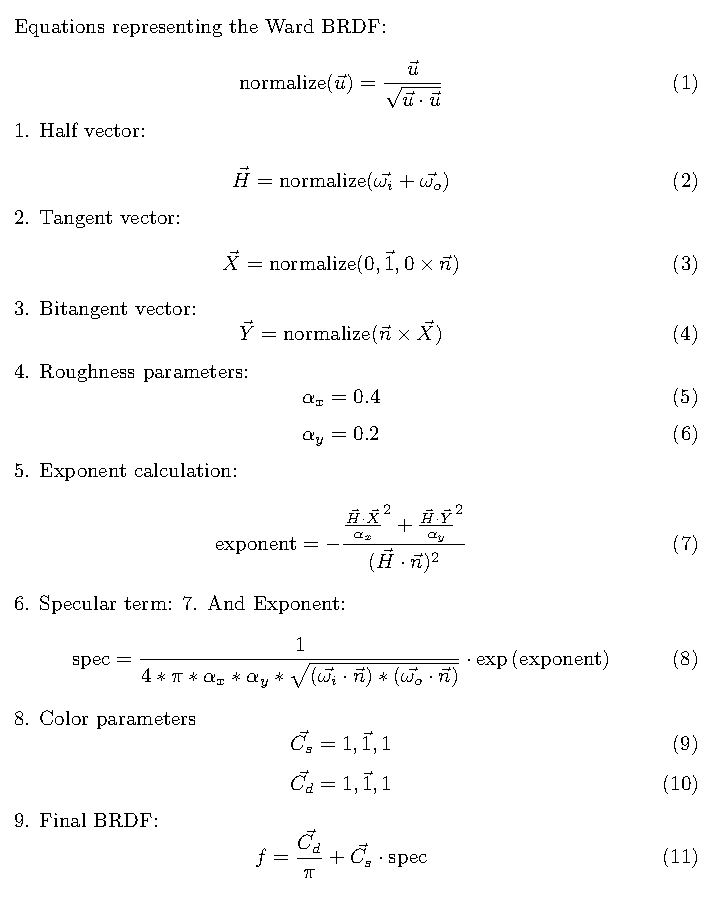
\includegraphics[scale=0.92]{./Imagens/brdfs/ward.pdf}
    \end{center}
\end{figure}

%%%%%%%%%%%%%%%%%%%%%%%%%%%%%%%%%%%%%%%%%%%%%%%%%
\subsection{Visualização do Resultado}
%%%%%%%%%%%%%%%%%%%%%%%%%%%%%%%%%%%%%%%%%%%%%%%%%
\begin{figure}[H]
    \caption{\small{Distribuição de Reflexão Especular e Difusa da BRDF}}\label{fig-ward-plots}
\minipage{0.48\textwidth}
    \vspace{42px}
  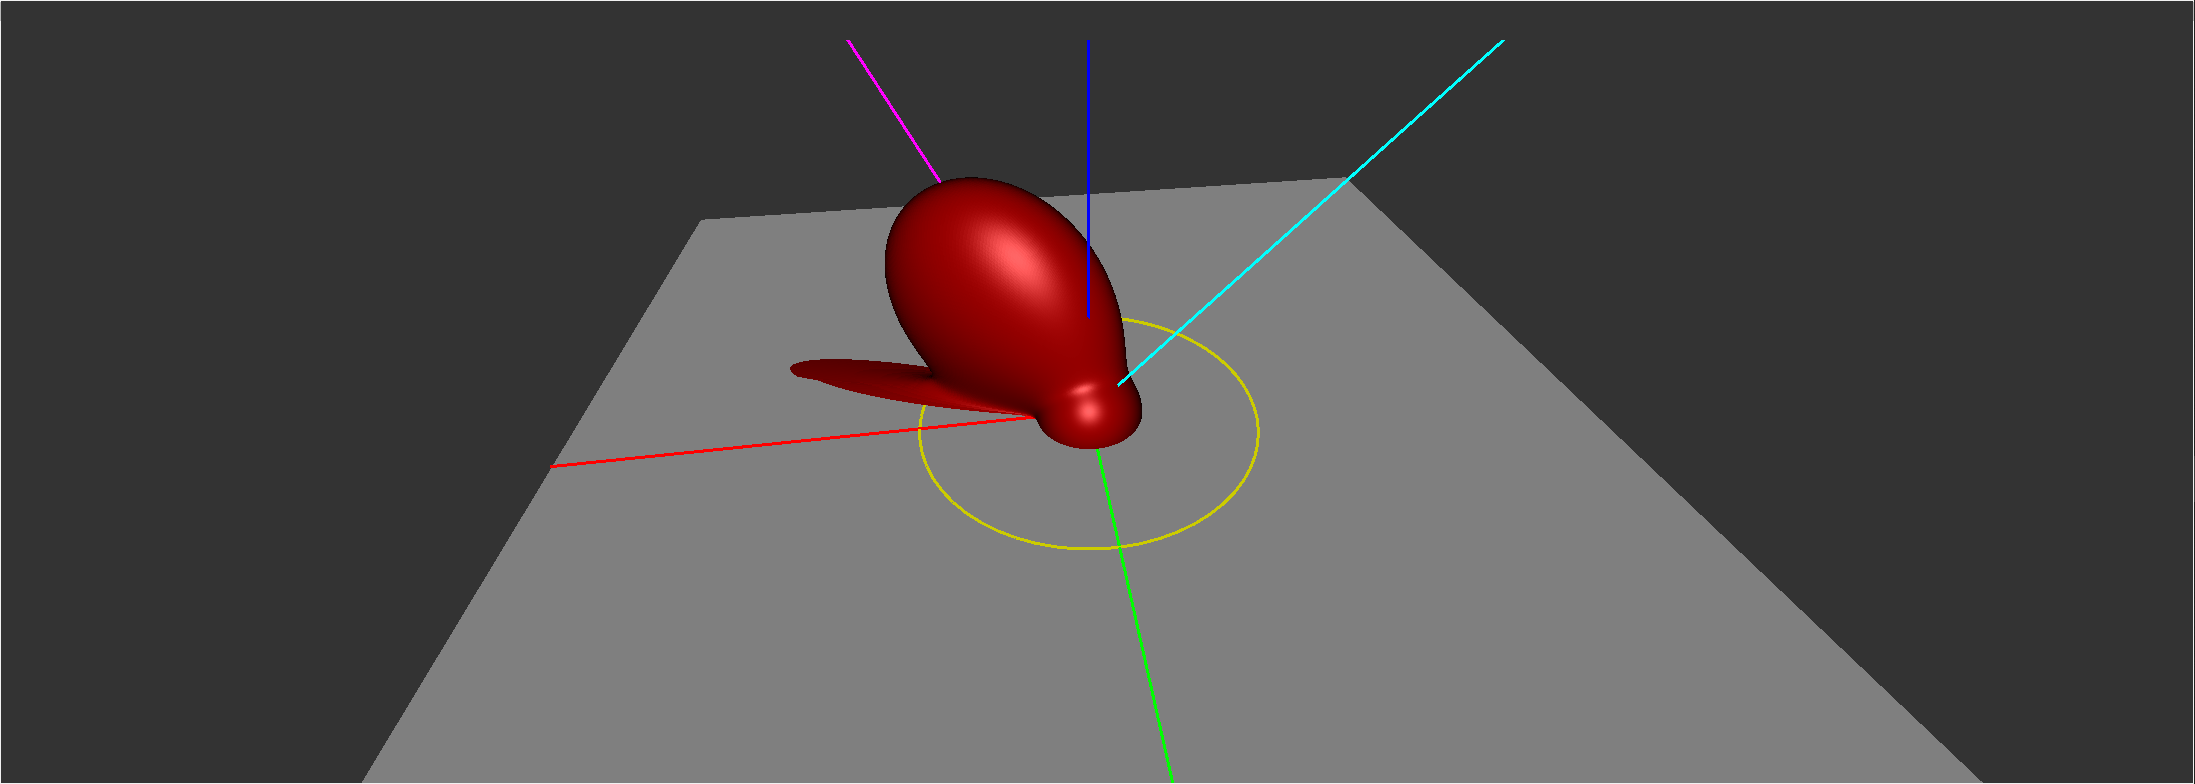
\includegraphics[width=\linewidth]{./Imagens/brdfs/ward-3D-plot}
    % \vspace{0.1px}
    \legend{ \small (a) 3D \textit{plot}}
\endminipage\hfill
\minipage{0.48\textwidth}
  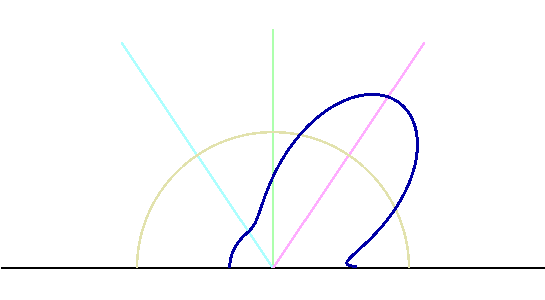
\includegraphics[width=\linewidth]{./Imagens/brdfs/ward-polar-plot.png}
    \legend{ \small (b) \textit{Polar plot}}
\endminipage\hfill
\end{figure}

\begin{figure}[H]
    \caption{\small{Objetos 3D renderizados por este experimento}}\label{fig-ward-objetcs}
\minipage{0.32\textwidth}
  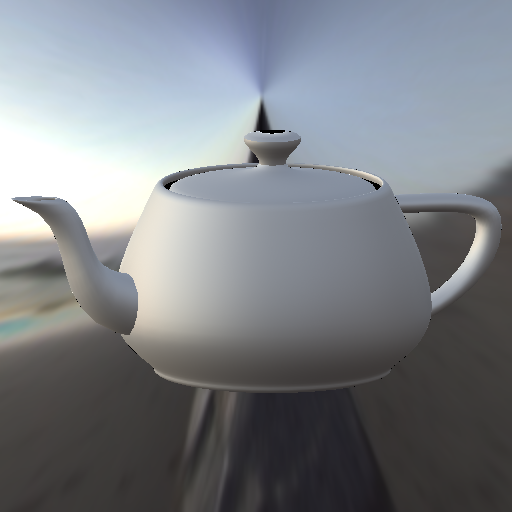
\includegraphics[width=\linewidth]{./Imagens/brdfs/ward-teapot.png}
    \legend{ \small (a) \textit{Teapot}}
\endminipage\hfill
\minipage{0.32\textwidth}
  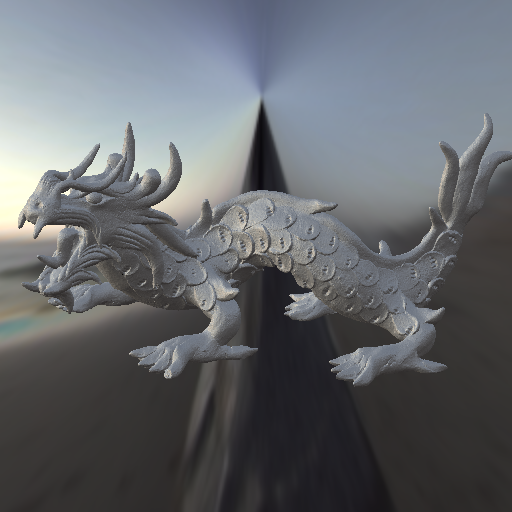
\includegraphics[width=\linewidth]{./Imagens/brdfs/ward-dragon.png}
    \legend{ \small (b) Dragão de Stanford}
\endminipage\hfill
\minipage{0.32\textwidth}%
  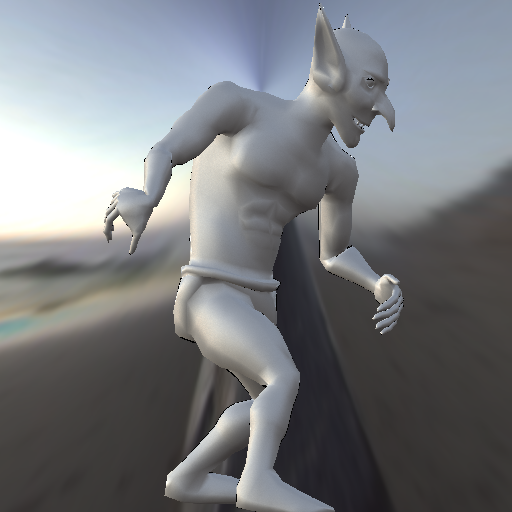
\includegraphics[width=\linewidth]{./Imagens/brdfs/ward-goblin.png}
    \legend{ \small (c) Goblin}
\endminipage
\end{figure}

%%%%%%%%%%%%%%%%%%%%%%%%%%%%%%%%%%%%%%%%%%%%%%%%%
\subsection{Código GLSL Gerado}
%%%%%%%%%%%%%%%%%%%%%%%%%%%%%%%%%%%%%%%%%%%%%%%%%
\begin{codigo}[H]
    \caption{\small Saida do compilador, código GLSL da BRDF deste experimento (parte 1). }
    \label{cod-ward-glsl-pt-1}
\begin{lstlisting}[language=C, inputencoding=utf8]
analytic
::begin parameters
#[type][name][min val][max val][default val]
::end parameters
::begin shader
//////////// START OF BUILTINS DECLARTION ////////////
vec3 var_0_vec_h;
vec3 var_3_vec_n;
float var_10_theta_h;
float var_11_theta_d;
float var_1_pi;
float var_2_epsilon;
vec3 var_4_vec_omega_i;
float var_5_theta_i;
float var_6_phi_i;
vec3 var_7_vec_omega_o;
float var_8_theta_o;
float var_9_phi_o;
//////////// END OF BUILTINS DECLARTION ////////////
//////////// START OF USER DECLARED ////////////
vec3 var_14_vec_X;
vec3 var_15_vec_Y;
float var_16_alpha_x;
float var_17_alpha_y;
vec3 var_18_vec_C_d;
vec3 var_19_vec_C_s;
vec3 var_20_vec_H;
float var_21_text_exponent;
float var_22_text_spec;
vec3 var_23_f;
//////////// END OF USER DECLARED ////////////
//////////// START FUNCTIONS DECLARATIONS ////////////
vec3 var_12_text_normalize(vec3 var_13_vec_u) {
  return (var_13_vec_u / sqrt(dot(var_13_vec_u, var_13_vec_u)));
}
//////////// END FUNCTIONS DECLARATIONS ////////////
\end{lstlisting}
\end{codigo}

\begin{codigo}[H]
    \caption{\small Saida do compilador, código GLSL da BRDF deste experimento  (parte 2). }
\label{cod-ward-glsl-pt-2}
\begin{lstlisting}[language=C, inputencoding=utf8]
vec3 BRDF(vec3 L, vec3 V, vec3 N, vec3 X, vec3 Y) {
  //////////// START OF BUILTINS INITIALIZATION ////////////
  var_0_vec_h = normalize(L + V);
  var_3_vec_n = normalize(N);
  var_1_pi = 3.141592653589793;
  var_2_epsilon = 1.192092896e-07;
  var_4_vec_omega_i = L;
  var_5_theta_i = atan(var_4_vec_omega_i.y, var_4_vec_omega_i.x);
  var_6_phi_i = atan(sqrt(var_4_vec_omega_i.y * var_4_vec_omega_i.y +
                          var_4_vec_omega_i.x * var_4_vec_omega_i.x),
                     var_4_vec_omega_i.z);
  var_7_vec_omega_o = V;
  var_8_theta_o = atan(var_7_vec_omega_o.y, var_7_vec_omega_o.x);
  var_9_phi_o = atan(sqrt(var_7_vec_omega_o.y * var_7_vec_omega_o.y +
                          var_7_vec_omega_o.x * var_7_vec_omega_o.x),
                     var_7_vec_omega_o.z);
  var_10_theta_h = acos(dot(var_0_vec_h, N));
  var_11_theta_d = acos(dot(var_0_vec_h, var_4_vec_omega_i));
  //////////// END OF BUILTINS INITIALIZATION ////////////
  var_14_vec_X = var_12_text_normalize(cross(vec3(0.0, 1.0, 0.0), var_3_vec_n));
  var_15_vec_Y = var_12_text_normalize(cross(var_3_vec_n, var_14_vec_X));
  var_16_alpha_x = 0.4;
  var_17_alpha_y = 0.2;
  var_18_vec_C_d = vec3(1.0, 1.0, 1.0);
  var_19_vec_C_s = vec3(1.0, 1.0, 1.0);
  var_20_vec_H = var_12_text_normalize((var_4_vec_omega_i + var_7_vec_omega_o));
  var_21_text_exponent = (-((pow((dot(var_20_vec_H, var_14_vec_X) / var_16_alpha_x), 2.0) +
          pow((dot(var_20_vec_H, var_15_vec_Y) / var_17_alpha_y), 2.0)) /
         pow((dot(var_20_vec_H, var_3_vec_n)), 2.0)));
  var_22_text_spec = ((1.0 / ((((4.0 * var_1_pi) * var_16_alpha_x) * var_17_alpha_y) *
               sqrt(((dot(var_4_vec_omega_i, var_3_vec_n)) *
                     (dot(var_7_vec_omega_o, var_3_vec_n)))))) *
       exp((var_21_text_exponent)));
  var_23_f = ((var_18_vec_C_d / var_1_pi) + (var_19_vec_C_s * var_22_text_spec));

  return vec3(var_23_f);
}
\end{lstlisting}
\end{codigo}

%%%%%%%%%%%%%%%%%%%%%%%%%%%%%%%%%%%%%%%%%%%%%%%%%
\subsection{Código Fonte em \texttt{EquationLang}}
%%%%%%%%%%%%%%%%%%%%%%%%%%%%%%%%%%%%%%%%%%%%%%%%%
\begin{codigo}[H]
    \caption{\small Código fonte da BRDF deste experimento (parte 1).}
    \label{cod-ward-eqlang-pt-1}
\begin{lstlisting}[language=tex, frame=none, inputencoding=utf8]
Equations representing the Ward BRDF:
   \begin{equation}
      \text{normalize}(\vec{u}) = \frac{\vec{u}}{\sqrt{\vec{u} \cdot \vec{u}}}
   \end{equation}
1. Half vector:
   \begin{equation}
   \vec{H} = \text{normalize}(\vec{\omega_i} + \vec{\omega_o})
   \end{equation}
2. Tangent vector:
   \begin{equation}
   \vec{X} = \text{normalize}(\vec{0,1,0} \times \vec{n})
   \end{equation}
3. Bitangent vector:
   \begin{equation}
   \vec{Y} = \text{normalize}(\vec{n} \times \vec{X})
   \end{equation}
4. Roughness parameters:
   \begin{equation}
   \alpha_x = 0.4
   \end{equation}
   \begin{equation}
   \alpha_y = 0.2
   \end{equation}
\end{lstlisting}
\end{codigo}

\begin{codigo}[H]
    \caption{\small Código fonte da BRDF deste experimento (parte 2).}
    \label{cod-ward-eqlang-pt-2}
\begin{lstlisting}[language=tex, frame=none, inputencoding=utf8]
5. Exponent calculation:
   \begin{equation}
   \text{exponent} = -\frac{
       \frac{\vec{H} \cdot \vec{X}}{\alpha_x}^2 +
       \frac{\vec{H} \cdot \vec{Y}}{\alpha_y}^2
   }{(\vec{H} \cdot \vec{n})^2}
   \end{equation}
6. Specular term:
7. And Exponent:
   \begin{equation}
   \text{spec} = \frac{1}{4*\pi * \alpha_x *\alpha_y *\sqrt{(\vec{\omega_i} \cdot \vec{n}) * (\vec{\omega_o} \cdot \vec{n})}}
      \cdot \exp{( \text{exponent} )}
   \end{equation}
8. Color parameters
   \begin{equation}
   \vec{C_s} = \vec{1, 1, 1}
   \end{equation}
   \begin{equation}
   \vec{C_d} = \vec{ 1, 1, 1 }
   \end{equation}
9. Final BRDF:
   \begin{equation}
   f = \frac{\vec{C_d}}{\pi} + \vec{C_s} \cdot \text{spec}
   \end{equation}
\end{lstlisting}
\end{codigo}
